\documentclass[12pt]{article}
\usepackage[a4paper,landscape,margin=1.5cm]{geometry} % Adjust margin as desired

% Packages for math symbols and functions
\usepackage{amsmath}
\usepackage{amssymb}
\usepackage{amsfonts}

% Package for rendering functions
\usepackage{mathrsfs}
\usepackage{pgfplots}
\usepackage{multicol}

% Adjust the font size for section headers
\usepackage{sectsty}
\sectionfont{\large\bfseries}

% Fancy Header
\usepackage{fancyhdr}
\pagestyle{fancy}
\fancyhf{} % Clear all header and footer fields
\lhead{\textsf{\textbf{HSLU Zulassungsstudium Formelsammlung}}}
\rhead{\textsf{Kevin Häusler}}
\title{\textsf{\textbf{HSLU Zulassungsstudium Formelsammlung}}}

% Tables
\usepackage{tabularx}

% Temp
\setlength{\columnseprule}{0.1pt} % Set the thickness of the line

% Define a command for displaying a function
\newcommand{\function}[2]{\ensuremath{\mathscr{#1}\left(#2\right)}}

% Define additional commands, if needed
% \newcommand{\commandname}{command definition}

\begin{document}


% Section Allgemein
%\section*{Allgemein}
\begin{multicols}{3}
\subsection*{Wachstum und Verfall}
\textbf{Wachtsumsfaktor:}
\begin{equation*}
    q = 100\ \% + p\ \% = 1 + \frac{p}{100}
\end{equation*} 
\textbf{Verdoppelungszeit:}
\begin{equation*}
    t_V = \frac{\ln(2)}{\ln(q)}
\end{equation*}
\textbf{Abnahme:}
\begin{equation*}
    B(t) = {\color{red}m} \cdot t + b \quad \text{mit } {\color{red}m < 0}
\end{equation*}

\subsection*{Summe und Produkte}
\textbf{Summezeichen:} \\
Es sei:  n, k $\in$ Z und n $\geq$ k
\begin{equation*}
    \sum_{k=1}^{n} a_k = a_1 + a_2 + a_3 + \ldots + a_n 
\end{equation*}
\textbf{Produktzeichen:}
\begin{equation*}
    \prod_{k=1}^{n} a_k = a_1 \cdot a_2 \cdot a_3 \cdot \ldots \cdot a_n
\end{equation*}
k = Laufvariable, Laufindex  \\
1 = Startwert  n = Endwert\\
$a_{k}$ ist die Funktion bezueglich der Laufvariable \\

\subsection*{Aussagen, Logik, Mengen}
\begin{tabularx}{\columnwidth} {
        | >{\raggedright\arraybackslash}c
        | >{\raggedright\arraybackslash}X |}
    \hline
    \textbf{*}            & \textbf{Bedeutung}                                           \\ \hline
    $\varnothing$ oder {} & Leere Menge                        \\ \hline
    $x\in A$              & Element x ist in Menge A                          \\ \hline
    $x\notin A$           & Element x ist nicht in Menge A                    \\ \hline
    $A\subset B$          & A ist eine Teilmenge von B                                   \\ \hline
    $A\cap B$             & Schnittmenge von A und B                                     \\ \hline
    $A\cup B$             & Vereinigunsgsmenge von A und B                               \\ \hline
    $A\backslash B$       & Differenzbildung, Menge A ohne B                         \\\hline
    $\bar{A}_B$           & $:= \{x \,|\, x \in B \enspace \wedge \enspace x \notin A\}$ \\\hline
\end{tabularx}


\def\firstcircle{(0,0) circle (1cm)}
    \def\secondcircle{(0:1.2cm) circle (1cm)}

    \colorlet{circle edge}{blue!50}
    \colorlet{circle area}{blue!20}

    \tikzset{filled/.style={fill=circle area, draw=circle edge, thick},
        outline/.style={draw=circle edge, thick}}

    \setlength{\parskip}{5mm}
    % Set A and B
    \begin{tikzpicture}
        \begin{scope}
            \clip \firstcircle;
            \fill[filled] \secondcircle;
        \end{scope}
        \draw[outline] \firstcircle node {$A$};
        \draw[outline] \secondcircle node {$B$};
        \node[anchor=south] at (current bounding box.north) {$A \cap B$};
    \end{tikzpicture}
    \begin{tikzpicture}
        \draw[filled] \firstcircle node {$A$}
        \secondcircle node {$B$};
        \node[anchor=south] at (current bounding box.north) {$A \cup B$};
    \end{tikzpicture}

    % Set A but not B
    \begin{tikzpicture}
        \begin{scope}
            \clip \firstcircle;
            \draw[filled, even odd rule] \firstcircle node {$A$}
            \secondcircle;
        \end{scope}
        \draw[outline] \firstcircle
        \secondcircle node {$B$};
        \node[anchor=south] at (current bounding box.north) {$A\backslash  B$};
    \end{tikzpicture}
    \begin{tikzpicture}
        \draw[filled, even odd rule] \firstcircle node {$A$}
        \secondcircle node{$B$};
        \node[anchor=south] at (current bounding box.north) {$\overline{A \cap B}$};
    \end{tikzpicture}\\
    \textbf{Aussagenlogik:}\\
    Eine Aussage beschreibt einen Sachverhalt (durch Worte oder Symbole), der
    entweder wahr oder falsch ist.\\

    \scriptsize
    \begin{tabular}{@{ }c@{ }@{ }c | c@{ }@{ }c@{ }@{ }c@{ }@{ }c@{ }@{ }c | c@{ }@{ }c@{ }@{ }c@{ }@{ }c@{ }@{ }c | c@{ }@{ }c | c@{ }@{ }c@{ }@{ }c@{ }@{ }c@{ }@{ }c@{ }@{ }c}
        A & B &  & A & $\land$            & B &  &  & A & $\lor$             & B &  & $\lnot$            & B &  & A & $\lor$             & $\lnot$ & B & \\
        \hline
        T & T &  & T & \textcolor{red}{T} & T &  &  & T & \textcolor{red}{T} & T &  & \textcolor{red}{F} & T &  & T & \textcolor{red}{T} & F       & T & \\
        T & F &  & T & \textcolor{red}{F} & F &  &  & T & \textcolor{red}{T} & F &  & \textcolor{red}{T} & F &  & T & \textcolor{red}{T} & T       & F & \\
        F & T &  & F & \textcolor{red}{F} & T &  &  & F & \textcolor{red}{T} & T &  & \textcolor{red}{F} & T &  & F & \textcolor{red}{F} & F       & T & \\
        F & F &  & F & \textcolor{red}{F} & F &  &  & F & \textcolor{red}{F} & F &  & \textcolor{red}{T} & F &  & F & \textcolor{red}{T} & T       & F & \\
    \end{tabular}
    \normalsize

    \begin{tabularx}{\columnwidth} {
        | >{\raggedright\arraybackslash}c
        | >{\raggedright\arraybackslash}X
        | >{\raggedright\arraybackslash}c|}
    \hline
    \textbf{*}            & \textbf{Bedeutung}                        & \textbf{Beispiel}             \\ \hline
    $|A|$                 & Kardinalität/Mächtigkeit      & A = {1;2}                     \\
                          & Anzahl Elemente               & |$|A|$ = 2                    \\ \hline
    $\land$               & Konkuktion/UND A $\land$    & A $\land$ B                   \\ \hline
    $\lor$                & Disjunktion/ODER A $\lor$ B  = Wahr wenn  & {-1;0;1;}                     \\\hline
    $\neg$                & Negation A = W $\neg$A = F      & $\neg $A                      \\\hline
    $\implies$            & Implikation: Daraus folgt                 &                               \\ \hline
    $\Longleftrightarrow$ & äquivalenz  &                               \\ \hline
    $\forall$             & für Alle                                  & $\forall$ $x \in \mathbb{N}$  \\ \hline
    $\exists$             & Es Existiert                              & $\exists $ $x \in \mathbb{N}$ \\ \hline
    \end{tabularx}
\subsection*{Misc}

\newpage
\end{multicols}



% Section Gleichungen


\section*{Gleichungen}

\begin{multicols*}{3}
\subsection*{Quadratische Gleichungen}
\textbf{Definiton} \\
Es gibt 4 Arten/Formen von Quadratischen Gleichungen.
\begin{enumerate}
    \item $ax^2 + bx + c = 0 \quad (a, b, c \in \mathbb{R}; a \neq 0)$
    \item $ax^2 + bx = 0 \quad (a, b \in \mathbb{R}; a \neq 0)$
    \item $ax^2 + c = 0 \quad (a, c \in \mathbb{R}; a \neq 0)$
    \item $ax^2 = 0 \quad (a \in \mathbb{R}; a \neq 0)$
\end{enumerate}
\subsubsection*{Lösung einer Reinquadratische Gleichung $ax^2 = 0$}
Reinquadratische Gleichungen ohne Absolutglied besitzen als einzige Lösung die Null.
\subsubsection*{Lösung einer Reinquadratische Gleichung mit Absolutglied $ax^2 + c = 0$}
Gleichung nach $x^2$ auflösen, Wurzel ziehen, Lösungsmenge aufschreiben.

\subsubsection*{Lösung einer Gemischtquadratische Gleichungen ohne Absolutglied $ax^2 + bx = 0$}
Quadratische Gleichung in Normalform bringen, $x$ ausklammern, Faktoren gleich Null setzen, Gleichung nach $x$ auflösen, Lösungsmenge aufschreiben.
\subsection*{Mitternachtsformel}
Gemischtquadratische Gleichungen $ax^2 + bx + c = 0$ mit Absolutglied lösen wir mit der Mitternachtsformel:
\[x_{1/2} = \frac{-b \pm \sqrt{b^2 - 4ac}}{2a}\]
\textbf{Fallunterscheidung:} \\
\begin{align*}
    x_{1} &= \dfrac{-b - \sqrt{b^2 - 4ac}}{2a} \\
    x_{2} &= \dfrac{-b + \sqrt{b^2 - 4ac}}{2a}
\end{align*}
\subsection*{Regeln}
Wenn das lineare Glied fehlt, gilt b = 0. \\
Wenn das absolute Glied fehlt, gilt c = 0. \\
Wenn das $x^2$ allein steht, gilt a = 0 (wegen $1 \cdot x^2 = x^2$).\\
Wenn das x allein steht, gilt b - 1(wegen $1 \cdot x = x$).
\subsection*{Lösen einer Quadratischen Gleichung mit Mitternachtsformel}
\begin{enumerate}
    \item Gleichung in allgemeine Form bringen
    \item a,b,c aus der allgemeinen Form herauslesen
    \item a,b,c in die Mitternachtsformel einsetzen
    \item Lösung berechnen
    \item Lösungsmenge aufschreiben
\end{enumerate}
\subsubsection*{Wurzelgleichungen}
\subsubsection*{Wurzelgesetze}
Wurzel Addieren = $a{\color{green}\sqrt[n]{x}} + b{\color{green}\sqrt[n]{x}} = (a + b){\color{green}\sqrt[n]{x}}$ \\
Wurzel Subtrahieren = $a {\color{green}\sqrt[n]{x}} - b{\color{green}\sqrt[n]{x}} = (a - b){\color{green}\sqrt[n]{x}}$ \\
Wurzel Multiplizieren = $\sqrt[{\color{green}n}]{a} \cdot \sqrt[{\color{green}n}]{b} = \sqrt[{\color{green}n}]{a \cdot b}$ \\
Wurzel Potenzieren = $(\sqrt[n]{a})^m = \sqrt[n]{a^m}$ \\
Wurzel Radizieren = $\sqrt[m]{\sqrt[n]{a}} = \sqrt[m \cdot n]{a}$ \\
Wurzel in Potenz umformen = $\sqrt[n]{a} = a^{\frac{1}{n}}$ oder $\sqrt[n]{a^m} = a^{\frac{m}{n}}$ \\
Wurzel Quadrieren: $\sqrt[]{a^2} = {(\sqrt[]{a})}^2 = a$ für $a \geq 0$ \\
Folgerung: $\sqrt[]{a^2} = |a|$
\subsubsection*{Wurzelgleichung lösen} 
Wurzel beseitigen (Wurzel isolieren, potenzieren), Gleichung lösen, Probe machen, Lösungsmenge aufschreiben.
\subsubsection*{Exponential und Logarithmusgleichungen}
\subsubsection*{Definition}
Eine Exponentialgleichung ist eine Gleichung, in der die Variable im Exponenten einer Potenz steht. \\
Eine Logarithmusgleichung ist eine Gleichung, in der die Variable im Numerus des Logarithmus steht.
\[a^{f(x)} = b^{g(x)} \quad \Rightarrow \quad f(x) \cdot \log a = g(x) \cdot \log b\]
Logarithmen mit der Basis e (der eulerschen Zahl) heissen natürliche Logarithmen.
\begin{equation*}
    e = \lim\limits_{n\rightarrow\infty}{\left(1+\frac{1}{n}\right)^n}.
\end{equation*}
$\exp{x} = e^x$ und $\ln{x}$ sind Kehrwertfunktionen
\begin{equation*}
    e^{\ln{x}} = x \text{ and } \ln{e^x} = x.
\end{equation*}
Exponentenregeln für Exponentengleichung
\begin{equation*}
    e^xe^y = e^{x+y} \text{, } \frac{e^x}{e^y}=e^{x-y} \text{, and } \left(e^x\right)^k=e^{xk}.
\end{equation*}
Exponentenregeln für Logarithmengleichung
\begin{equation*}
    \begin{aligned}
        \ln{x}+\ln{y} = \ln{xy} \text{, } \ln{x}-\ln{y} = \\
        \ln{\left(\frac{x}{y}\right)} \text{, and } \ln{\left(a^b\right)} = b\ln{a}.
    \end{aligned}
\end{equation*}
Wir können auch einen Logarithmus jeder Basis schreiben, indem wir natürliche Logarithmen verwenden:
\begin{equation*}
    \log_{b}{a} = \frac{\ln{a}}{\ln{b}}.
\end{equation*}
\textbf{Lösung des Logarithmus}\\
Eine Lösung mithilfe der Definition des Logarithmus ist nur dann möglich, wenn es gelingt, die Terme auf beiden Seiten der Gleichung so umzuformen, dass sich auf der einen Seite ein Logarithmus und auf der anderen Seite eine Konstante ergeben.\\
\textbf{Definitionsmenge Logarithmusgleichung }\\
Da $\log_{b}x = a$  nur für $x > 0$ definiert ist, kann die Definitionsmenge eingeschränkt sein.
In der Praxis bedeutet das, dass wir stets die Probe machen sollten, d.h. überprüfen, ob die berechneten Lösungen eingesetzt in die gegebene Gleichung zu einer wahren Aussage führen.\\
\subsubsection*{Logarithmengesetze}
Produktregel: $\log_b(P \cdot Q) = \log_b P + \log_b Q$ \\
Quotientregel: $\log_b\left(\frac{P}{Q}\right) = \log_b P - \log_b Q$ \\
Potenzregel 1: $\log_b P^n = n \cdot \log_b P$ \\
Potenzregel 2: $\log_b \sqrt[n]{P} = \frac{\log_b P}{n}$ \\
Basiswechsel: $\log_a P = \frac{\log_b P}{\log_b a}$    
\subsection*{Ungleichungen}
\subsubsection*{Rechenregeln}
    $ a < b \quad \Longleftrightarrow \quad b > a$\\
    $a \leq b \quad \Rightarrow \quad a+c \leq b+c$\\
    $a \leq b \quad\text{und}\quad c \leq d \quad \Rightarrow \quad a+c \leq b+d$\\
    $a < b \quad\text{und}\quad c \leq d \quad \Rightarrow \quad a+c < b+d$\\
    $a \leq b \quad\text{und}\quad c \geq 0 \quad \Rightarrow \quad ac \leq bc$\\
    $a \leq b \quad\text{und}\quad c \leq 0 \quad \Rightarrow \quad ac \geq bc$
    $a \leq b \quad \Rightarrow \quad \frac{1}{a} \geq \frac{1}{b}$
    \subsubsection*{Quadratische Ungleichungen}
    Eine Ungleichung, die sich durch Äquivalenzumformungen in eine der Formen bringen lässt, heisst quadratische Ungleichung.\\
    $ax^2 + bx + c < 0$\\
    $ax^2 + bx + c > 0$\\
    $ax^2 + bx + c \leq 0$\\
    $ax^2 + bx + c \geq 0$\\
    \begin{enumerate}
        \item Quadratische Gleichung lösen
        \item Potenzielle Lösungsintervalle aufstellen
        \item Überprüfen, welche Lösungsintervalle zur Lösung gehören
    \end{enumerate}
    Eine quadratische Gleichung besitzt entweder keine Lösung, eine Lösung oder zwei Lösungen.
    \subsubsection*{Bruchungleichungen}
    Bei Bruchungleichungen gibt es 2 Fälle:
    \textbf{Rechte Seite der Ungleichung $\neq$ 0}
    \begin{enumerate}
        \item Bruch durch Fallunterscheidung auflösen
        \item Lösungsmengen der einzelnen Fälle bestimmen (Intervalle)
        \item Lösungsmenge der Bruchungleichung bestimmen
    \end{enumerate}
    \begin{equation*} \frac{\text{Z}}{\text{N}} > c = \begin{cases} \frac{\text{Z}}{\text{N}} \cdot \text{N} > c \cdot \text{N} &\text{für } \text{N} > 0 \\[5px] \frac{\text{Z}}{\text{N}} \cdot \text{N} < c \cdot \text{N} &\text{für } \text{N} < 0 \end{cases} \end{equation*}
    Das Auflösen des Bruchs geschieht durch Multiplikation der Ungleichung mit dem Nenner des Bruchs. Dabei müssen wir jedoch eine Fallunterscheidung vornehmen. Ist der Nenner nämlich negativ, dreht sich das Ungleichheitszeichen um.
    \begin{equation*} \frac{\text{Z}}{\text{N}} > c = \begin{cases} \text{Z} > c \cdot \text{N} &\text{für } \text{N} > 0 \\[5px] \text{Z} < c \cdot \text{N} &\text{für } \text{N} < 0 \end{cases} \end{equation*}
    Die Lösungsmenge der Ungleichung ist die Vereinigungsmenge der einzelnen Lösungsmengen.
    \textbf{Rechte Seite der Ungleichung = 0}
    \begin{enumerate}
        \item Definitionsbereich bestimmen
        \item Nullstellen berechnen
        \item Intervallweise Betrachtung
    \end{enumerate}
\end{multicols*}



% Section Funtkionen
\section*{Funktionen}
\small
\begin{multicols}{3}
    \subsection*{Lineare Funktion}
    \begin{center}
        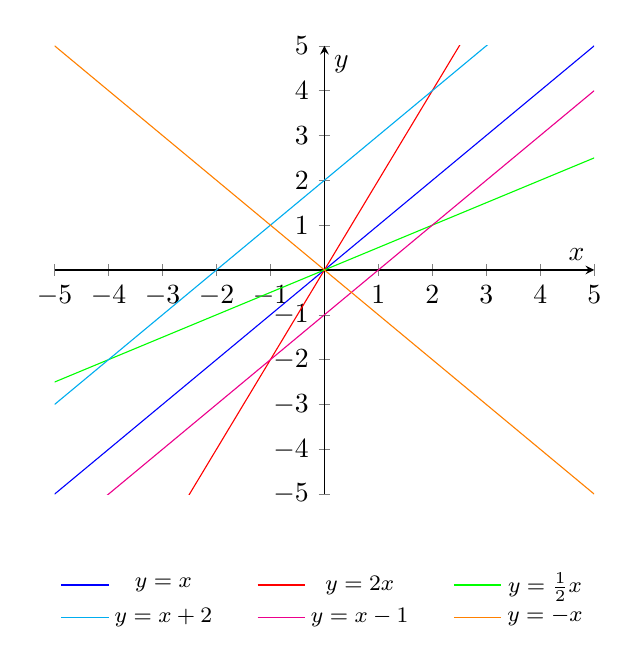
\begin{tikzpicture}
        \begin{axis}[
            axis lines=middle,
            xlabel=$x$,
            ylabel=$y$,
            xmin=-5,
            xmax=5,
            ymin=-5,
            ymax=5,
            xtick={-5,-4,-3,-2,-1,0,1,2,3,4,5},
            ytick={-5,-4,-3,-2,-1,0,1,2,3,4,5},
            legend pos=outer north east,
            legend style={
                draw=none,
                at={(0.5,-0.15)},
                anchor=north,
                legend columns=3,
                font=\footnotesize,
                /tikz/every even column/.append style={column sep=0.5cm},
            },
        ]
        
        % Linear Function: y = x
        \addplot[blue, domain=-5:5, samples=100] {x};
        \addlegendentry{$y = x$}
        
        % Transformed Functions
        \addplot[red, domain=-5:5, samples=100] {2*x};
        \addlegendentry{$y = 2x$}
        
        \addplot[green, domain=-5:5, samples=100] {0.5*x};
        \addlegendentry{$y = \frac{1}{2}x$}
        
        \addplot[cyan, domain=-5:5, samples=100] {x + 2};
        \addlegendentry{$y = x + 2$}
        
        \addplot[magenta, domain=-5:5, samples=100] {x - 1};
        \addlegendentry{$y = x - 1$}

        \addplot[orange, domain=-5:5, samples=100] {-x};
        \addlegendentry{$y = -x$}
        
        \end{axis}
        \end{tikzpicture}
    \end{center}
    \textbf{Definitonsmenge}: $\mathbb{D} = \mathbb{R}$\\
    \textbf{Wertemenge}: $\mathbb{W} = \mathbb{R}$\\
    \textbf{Nullstelle berechnen}\\
    Funktion gleich Null setzen und nach X auflösen.\\
    \textbf{Achsenabschnitt}:\\
    Bei linearen Funktionen lässt sich der y-Achsenabschnitt aus der Funktionsgleichung ablesen: Der y-Achsenabschnitt $y = {\color{red}mx + b}$ von ist $y = {\color{red}b}$\\
    \textbf{Schnittpunkt berechnen}\\
    Beide Funktionen gleichsetzen, nach X auflösen und in eine der beiden Funktionen einsetzen um Y zu berechnen.\\
    \textbf{Umkehrfunktion bilden}\\
    Funktion nach x auflösen, x und y vertauschen.\\
   
% Quadratic Function: y = x^2
\subsection*{Quadratische Funktion}
\begin{center}
    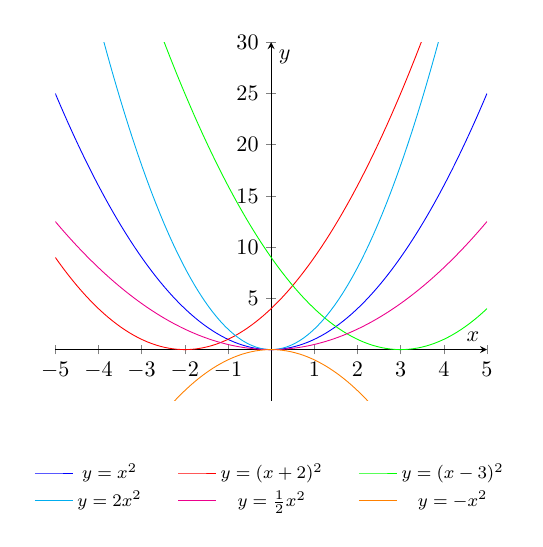
\begin{tikzpicture}[scale=0.8]
    \begin{axis}[
        axis lines=middle,
        xlabel=$x$,
        ylabel=$y$,
        xmin=-5,
        xmax=5,
        ymin=-5,
        ymax=30,
        xtick={-5,-4,-3,-2,-1,0,1,2,3,4,5},
        ytick={0,5,10,15,20,25,30},
        legend pos=outer north east,
            legend style={
                draw=none,
                at={(0.5,-0.15)},
                anchor=north,
                legend columns=3,
                font=\footnotesize,
                /tikz/every even column/.append style={column sep=0.5cm},
            },
    ]
    \addplot[blue, domain=-5:5, samples=100] {x^2};
    \addlegendentry{$y = x^2$}
    
    % Transformed Functions
    \addplot[red, domain=-5:5, samples=100] {(x+2)^2};
    \addlegendentry{$y = (x + 2)^2$}
    
    \addplot[green, domain=-5:5, samples=100] {(x-3)^2};
    \addlegendentry{$y = (x - 3)^2$}
    
    \addplot[cyan, domain=-5:5, samples=100] {2*x^2};
    \addlegendentry{$y = 2x^2$}
    
    \addplot[magenta, domain=-5:5, samples=100] {0.5*x^2};
    \addlegendentry{$y = \frac{1}{2}x^2$}

    \addplot[orange, domain=-5:5, samples=100] {-x^2};
    \addlegendentry{$y = -x^2$}
    
    \end{axis}
    \end{tikzpicture}
    \end{center}
    \textbf{Definitonsmenge}: $\mathbb{D} = \mathbb{R}$\\
    \textbf{Wertemenge}: $\mathbb{W} = \{y \in \mathbb{R} | y \geq 0\}$\\
    Der Graph einer quadratischen Funktion ist eine Parabel.
    Der tiefste oder höchste Punkt einer Parabel heisst Scheitelpunkt.\\
    \textbf{Achsenabschnitt}:\\
    Die x-Koordinate des Schnittpunktes mit der y-Achse ist immer Null.
    Bei quadratischen Funktionen lässt sich der y-Achsenabschnitt aus der Funktionsgleichung ablesen: Der y-Achsenabschnitt $y = ax^2 + bx + {\color{red}c}$ von ist $y = {\color{red}c}$
    \textbf{Nullstellen berechnen}:\\
    Funktionsgleichung gleich Null setzen, Gleichung lösen.
    
    % Exponential Function: y = 2^x
    \subsection*{Exponential Funktion}
    \begin{center}
    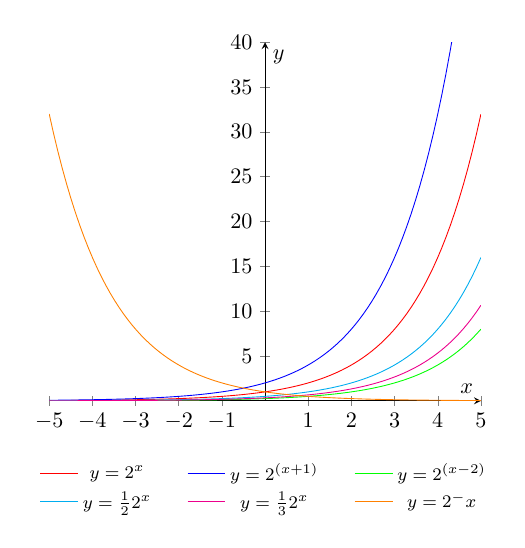
\begin{tikzpicture}[scale=0.8]
    \begin{axis}[
        axis lines=middle,
        xlabel=$x$,
        ylabel=$y$,
        xmin=-5,
        xmax=5,
        ymin=0,
        ymax=40,
        xtick={-5,-4,-3,-2,-1,0,1,2,3,4,5},
        ytick={0,5,10,15,20,25,30,35,40},
        legend pos=outer north east,
            legend style={
                draw=none,
                at={(0.5,-0.15)},
                anchor=north,
                legend columns=3,
                font=\footnotesize,
                /tikz/every even column/.append style={column sep=0.5cm},
            },
    ]
    \addplot[red, domain=-5:5, samples=100] {2^x};
    \addlegendentry{$y = 2^x$}
    
    % Transformed Functions
    \addplot[blue, domain=-5:5, samples=100] {2^(x+1)};
    \addlegendentry{$y = 2^{(x + 1)}$}
    
    \addplot[green, domain=-5:5, samples=100] {2^(x-2)};
    \addlegendentry{$y = 2^{(x - 2)}$}
    
    \addplot[cyan, domain=-5:5, samples=100] {0.5*2^x};
    \addlegendentry{$y = \frac{1}{2}2^x$}
    
    \addplot[magenta, domain=-5:5, samples=100] {2^x / 3};
    \addlegendentry{$y = \frac{1}{3}2^x$}

    \addplot[orange, domain=-5:5, samples=100] {2^-x};
    \addlegendentry{$y = 2^-x$}
    
    \end{axis}
    \end{tikzpicture}
    \end{center}
    \textbf{Definitonsmenge}: $\mathbb{D} = \mathbb{R}$\\
    \textbf{Wertemenge}: $\mathbb{W} = \mathbb{R^+}$\\
    \textbf{Basis a zwisschen 0 und 1}\\
    Gilt $0 < a < 1$, so ist die Exponentialfunktion streng monoton fallend. Exponentialler Abnahme.\\
    \textbf{Basis a grösser 1}\\
    Gilt $a > 1$, so ist die Exponentialfunktion streng monoton wachsend. Exponentielles Wachstum.\\
    \textbf{Eigenschaften}\\
    Der Graph einer Exponentialfunktion verläuft durch den Punkt $(0;1)$.\\
    Die Exponentialfunktion hat keine Nullstelle.\\
    Die x-Achse ist eine waagrechte Asymptote die beliebig nah an den Nullpunkt kommt.\\
    \textbf{Umkehrfunktion}\\
    Die Umkehrfunktion der Exponentialfunktion heisst Logarithmusfunktion. $f(x) = \log_{a}x$\\ 
        
    \subsection*{Logarithmische Funktion}
    % Logarithmic Function: y = ln(x)
    \begin{center}
    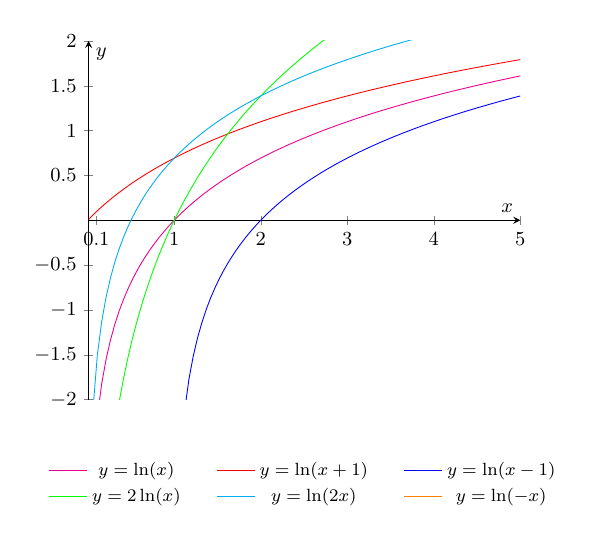
\begin{tikzpicture}[scale=0.8]
    \begin{axis}[
        axis lines=middle,
        xlabel=$x$,
        ylabel=$y$,
        xmin=0.01,
        xmax=5,
        ymin=-2,
        ymax=2,
        xtick={0.01,0.1,1,2,3,4,5},
        ytick={-2,-1.5,-1,-0.5,0,0.5,1,1.5,2},
        legend pos=outer north east,
            legend style={
                draw=none,
                at={(0.5,-0.15)},
                anchor=north,
                legend columns=3,
                font=\footnotesize,
                /tikz/every even column/.append style={column sep=0.5cm},
            },
    ]
    \addplot[magenta, domain=0.01:5, samples=100] {ln(x)};
    \addlegendentry{$y = \ln(x)$}
    
    % Transformed Functions
    \addplot[red, domain=0.01:5, samples=100] {ln(x+1)};
    \addlegendentry{$y = \ln(x + 1)$}
    
    \addplot[blue, domain=0.01:5, samples=100] {ln(x-1)};
    \addlegendentry{$y = \ln(x - 1)$}
    
    \addplot[green, domain=0.01:5, samples=100] {2*ln(x)};
    \addlegendentry{$y = 2\ln(x)$}
    
    \addplot[cyan, domain=0.01:5, samples=100] {ln(2*x)};
    \addlegendentry{$y = \ln(2x)$}

    \addplot[orange, samples=100] {ln(-x)};
    \addlegendentry{$y = \ln(-x)$}
    \small
    \end{axis}
    \end{tikzpicture}
    \end{center}
    \textbf{Definitonsmenge}: $\mathbb{D} = \mathbb{R^+}$\\
    \textbf{Wertemenge}: $\mathbb{W} = \mathbb{R}$\\
    \textbf{Basis a zwisschen 0 und 1}\\
    Gilt $0 < a < 1$, so ist die Exponentialfunktion streng monoton fallend.\\
    \textbf{Basis a grösser 1}\\
    Gilt $a > 1$, so ist die Exponentialfunktion streng monoton wachsend. Exponentielles Wachstum.\\
    \textbf{Eigenschaften}\\
    Logarithmuskurven verlaufen durch den Punkt $(1;0)$.    Die Nullstellen der Logarithmusfunktionen ist x=1.\\
    Logarithmuskurven verlaufen rechts der y-Achse.\\
    Logarithmusfunktionen haben keinen y-Achsenabschnitt.\\
    Die y-Achse ist eine senkrechte Asymptote die beliebig nah an den Nullpunkt kommt.\\
    \subsection*{Potenz Funktion}
    \subsubsection*{Potenzfunktionen mit Positiven Exponenten}
    \subsubsection*{Definition}
    Eine Funktion $f$ mit der Funktionsgleichung $f(x) = x^n \quad \text{ mit } n \in \mathbb{Z}\setminus\{0\}$ heisst Potenzfunktion. \\~\\
    \subsubsection*{Gerade Exponenten}
    Als Beispiele dienen die Funktionen $f(x) = x^2$ und $f(x) = x^4$. \\
    Um die Graphen besser zu zeichnen, berechnen wir zunächst einige Funktionswerte:
    \[\begin{array}{r|c|c|c|c|c|c|c} x & -1{,}5 & {\color{blue}-1} & -0{,}5 & {\color{blue}0} & 0{,}5 & {\color{blue}1} & 1{,}5 \\ \hline x^2 & 2{,}25 & {\color{blue}1} & 0{,}25 & {\color{blue}0} & 0{,}25 & {\color{blue}1} & 2{,}25 \\ \hline x^4 & 5{,}0625 & {\color{blue}1} & 0{,}0625 & {\color{blue}0} & 0{,}0625 & {\color{blue}1} & 5{,}0625 \end{array}\]
    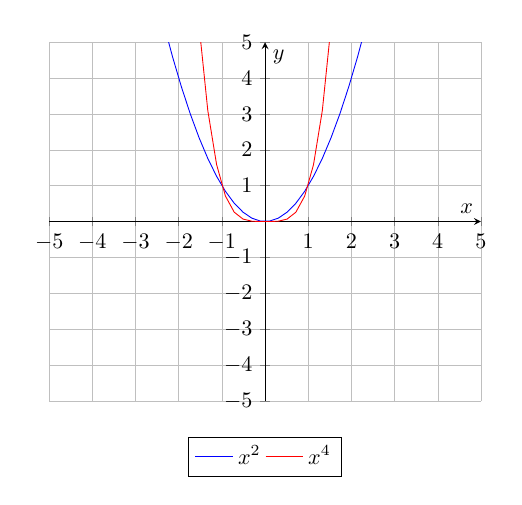
\begin{tikzpicture}[scale=0.8]
        \begin{axis}[
                xlabel=$x$,
                ylabel=$y$,
                xmax=5,
                xmin=-5,
                ymax=5,
                ymin=-5,
                axis x line=middle,
                axis y line=middle,
                legend style={at={(0.5,-0.1)},
                        anchor=north,legend columns=-1},
                grid=major,
                grid style={line width=.1pt, draw=gray!10},
                major grid style={line width=.2pt,draw=gray!50},
                xtick={-5,-4,-3,-2,-1,0,1,2,3,4,5},
                ytick={-5,-4,-3,-2,-1,0,1,2,3,4,5},
                samples=50
            ]
            \addplot [blue] {x^2};
            \addlegendentry {$x^2$};
            \addplot [red] {x^4};
            \addlegendentry {$x^4$};


        \end{axis}
    \end{tikzpicture}
    \subsubsection*{Ungerade Exponenten}
    Als Beispiele dienen die Funktionen $f(x) = x^3$ und $f(x) = x^5$. \\
    Um die Graphen besser zu zeichnen, berechnen wir zunächst einige Funktionswerte:  \\
    \footnotesize
    \[\begin{array}{r|c|c|c|c|c|c|c} x & -1{,}5 & {\color{blue}-1} & -0{,}5 & {\color{blue}0} & 0{,}5 & {\color{blue}1} & 1{,}5 \\ \hline x^3 & -3{,}375 & {\color{blue}-1} & -0{,}125 & {\color{blue}0} & 0{,}125 & {\color{blue}1} & 3{,}375 \\ \hline x^5 & -7{,}59375 & {\color{blue}-1} & 0{,}03125 & {\color{blue}0} & 0{,}03125 & {\color{blue}1} & 7{,}59375 \end{array}\]
    \normalsize
    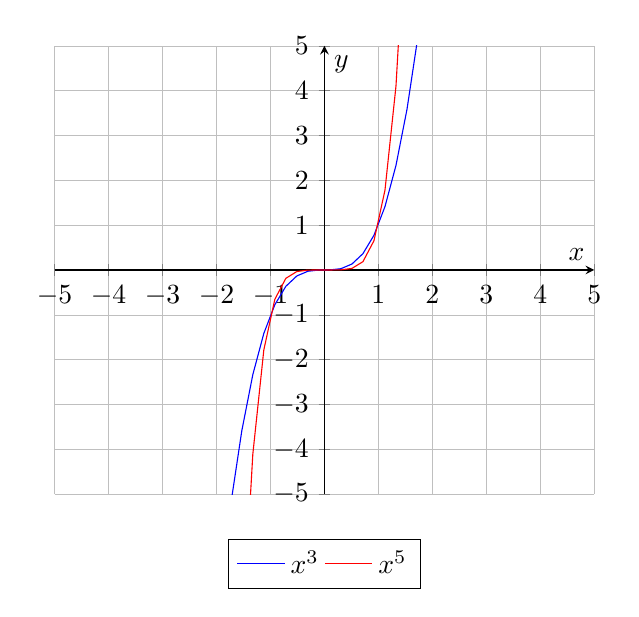
\begin{tikzpicture}%[scale=1.5]
        \begin{axis}[
                xlabel=$x$,
                ylabel=$y$,
                xmax=5,
                xmin=-5,
                ymax=5,
                ymin=-5,
                restrict y to domain=-10:10,
                axis x line=middle,
                axis y line=middle,
                legend style={at={(0.5,-0.1)},
                        anchor=north,legend columns=-1},
                grid=major,
                grid style={line width=.1pt, draw=gray!10},
                major grid style={line width=.2pt,draw=gray!50},
                xtick={-5,-4,-3,-2,-1,0,1,2,3,4,5},
                ytick={-5,-4,-3,-2,-1,0,1,2,3,4,5},
                samples=50
            ]
            \addplot [blue] {x^3};
            \addlegendentry {$x^3$};
            \addplot [red] {x^5};
            \addlegendentry {$x^5$};
        \end{axis}
    \end{tikzpicture}

    \subsubsection*{Zusammenfassung der wichtigsten Eigenschaften}
    Potenzfunktionen mit positiven ganzzahligen Exponenten $\boldsymbol{f(x) = x^n}$ haben folgende Eigenschaften: \\
    \begin{tabularx}{\columnwidth} {
            | >{\raggedright\arraybackslash}X
            | >{\raggedright\arraybackslash}X
            | >{\raggedright\arraybackslash}X |}
        \hline
                          & \textbf{n gerade}                 & \textbf{n ungerade}       \\ \hline
        D-Menge  & $\mathbb{D} = \mathbb{R}$         & $\mathbb{D} = \mathbb{R}$ \\ \hline
        Wertemenge        & $\mathbb{W} = \mathbb{R}^{+}_{0}$ & $\mathbb{W} = \mathbb{R}$ \\ \hline
        Symmetrie         & achsen                 & punkt           \\
                          & zur y-ache                        & zum K-Ursprung            \\ \hline
        Gemeinsame  & $(-1,1)$,$(0|0)$,      & $(-1,-1)$,$(0|0)$, \\ 
        Punkte& $(1|1)$          & $(1|1)$ \\ \hline
    \end{tabularx}
    \subsection*{Potenzfunktionen mit negativen Exponenten}
    Die Graphen von Potenzfunktionen heissen Hyperbeln n-ter Ordnung, wenn der Exponent negativ ist.
    \subsubsection*{Gerade Exponenten}
     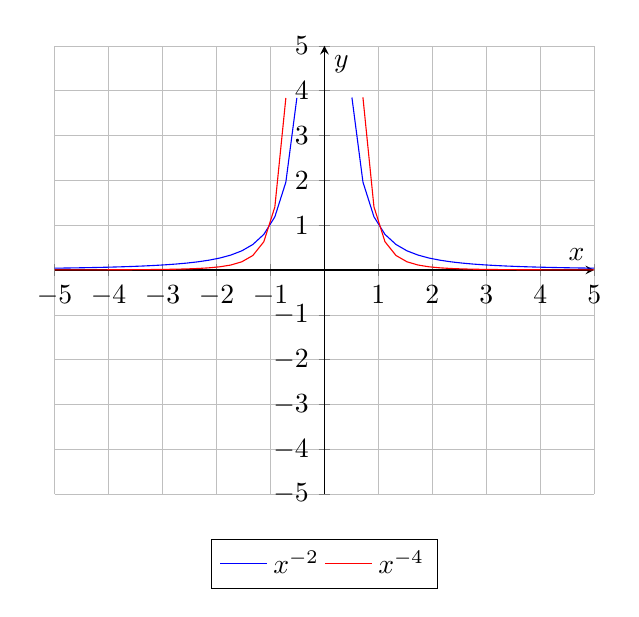
\begin{tikzpicture}[scale=1]
        \begin{axis}[
                xlabel=$x$,
                ylabel=$y$,
                xmax=5,
                xmin=-5,
                ymax=5,
                ymin=-5,
                restrict y to domain=-10:10,
                axis x line=middle,
                axis y line=middle,
                legend style={at={(0.5,-0.1)},
                        anchor=north,legend columns=-1},
                grid=major,
                grid style={line width=.1pt, draw=gray!10},
                major grid style={line width=.2pt,draw=gray!50},
                xtick={-5,-4,-3,-2,-1,0,1,2,3,4,5},
                ytick={-5,-4,-3,-2,-1,0,1,2,3,4,5},
                samples=50
            ]
            \addplot [blue] {x^-2};
            \addlegendentry {$x^{-2}$};
            \addplot [red] {x^-4};
            \addlegendentry {$x^{-4}$};
        \end{axis}
    \end{tikzpicture}\\
    Als Beispiele dienen die Funktionen $f(x) = x^{-2}$ und $f(x) = x^{-4}$. \\
    Um die Graphen besser zu zeichnen, berechnen wir zunächst einige Funktionswerte: \\~\\
    $\begin{array}{r|c|c|c|c|c|c} x & -1{,}5 & {\color{blue}-1} & -0{,}5 & 0{,}5 & {\color{blue}1} & 1{,}5 \\ \hline x^{-2} & 0{,}\bar{4} & {\color{blue}1} & 4 & 4 & {\color{blue}1} & 0{,}\bar{4} \\ \hline x^{-4} & \approx 0{,}1975 & {\color{blue}1} & 16 & 16 & {\color{blue}1} & \approx 0{,}1975 \end{array}$ \\~\\
    \small
    \subsubsection*{Gerade Exponenten}
    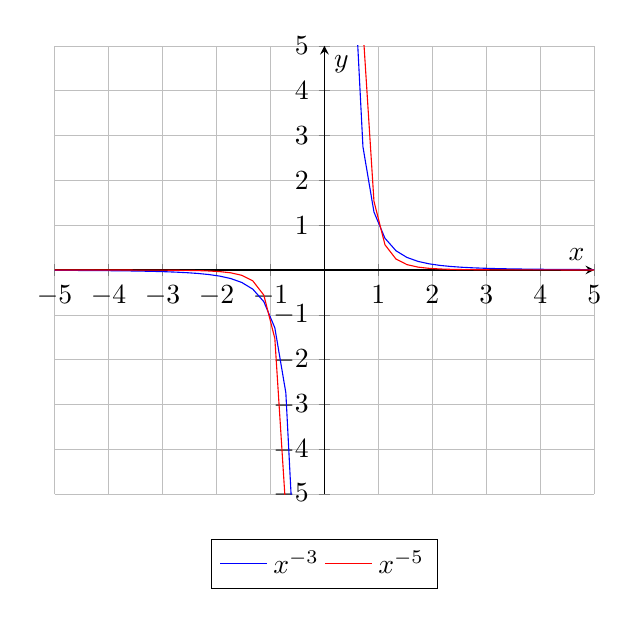
\begin{tikzpicture}[scale=1]
        \begin{axis}[
                xlabel=$x$,
                ylabel=$y$,
                xmax=5,
                xmin=-5,
                ymax=5,
                ymin=-5,
                restrict y to domain=-10:10,
                axis x line=middle,
                axis y line=middle,
                legend style={at={(0.5,-0.1)},
                        anchor=north,legend columns=-1},
                grid=major,
                grid style={line width=.1pt, draw=gray!10},
                major grid style={line width=.2pt,draw=gray!50},
                xtick={-5,-4,-3,-2,-1,0,1,2,3,4,5},
                ytick={-5,-4,-3,-2,-1,0,1,2,3,4,5},
                samples=50
            ]
            \addplot [blue] {x^-3};
            \addlegendentry {$x^{-3}$};
            \addplot [red] {x^-5};
            \addlegendentry {$x^{-5}$};
        \end{axis}
    \end{tikzpicture}\\
    Als Beispiele dienen die Funktionen $f(x) = x^{-3}$ und $f(x) = x^{-5}$. \\
    Um die Graphen besser zu zeichnen, berechnen wir zunächst einige Funktionswerte: \\~\\
    $\begin{array}{r|c|c|c|c|c|c} x & -1{,}5 & {\color{blue}-1} & -0{,}5 & 0{,}5 & {\color{blue}1} & 1{,}5 \\ \hline x^{-3} & \approx -0{,}2963 & {\color{blue}-1} & -8 & 8 & {\color{blue}1} & \approx 0{,}2963 \\ \hline x^{-5} & \approx -0{,}1317 & {\color{blue}-1} & -32 & 32 & {\color{blue}1} & \approx 0{,}1317 \end{array}$ \\~\\
 

    \subsubsection*{Zusammenfassung der wichtigsten Eigenschaften}
    Potenzfunktionen mit negativen ganzzahligen Exponenten $\boldsymbol{f(x) = x^{-n}}$ haben folgende Eigenschaften: \\\\
    \begin{tabularx}{\columnwidth} {
            | >{\raggedright\arraybackslash}X
            | >{\raggedright\arraybackslash}X
            | >{\raggedright\arraybackslash}X |}
        \hline
                          & \textbf{n gerade}                       & \textbf{n ungerade}                     \\ \hline
        D-Menge  & $\mathbb{D} = \mathbb{R}\setminus\{0\}$ & $\mathbb{D} = \mathbb{R}\setminus\{0\}$ \\ \hline
        Wertemenge        & $\mathbb{W} = \mathbb{R}^{+}$           & $\mathbb{W} = \mathbb{R}\setminus\{0\}$ \\ \hline
        Symmetrie         & achsen                       & punkt                         \\
                          & zur y-ache                              & zum K-Ursprung                          \\ \hline
        Gemeinsame Punkte & $(-1,1)$,$(1|1)$                        & $(-1,-1)$,$(1|1)$                       \\ \hline
        Asymptoten        & x-Achse, y-Achse                        & x-Achse, y-Achse                        \\ \hline
    \end{tabularx}


    
    \subsection*{Wurzel Funktion}
    % Square Root Function: y = sqrt(x)
    \begin{center}
    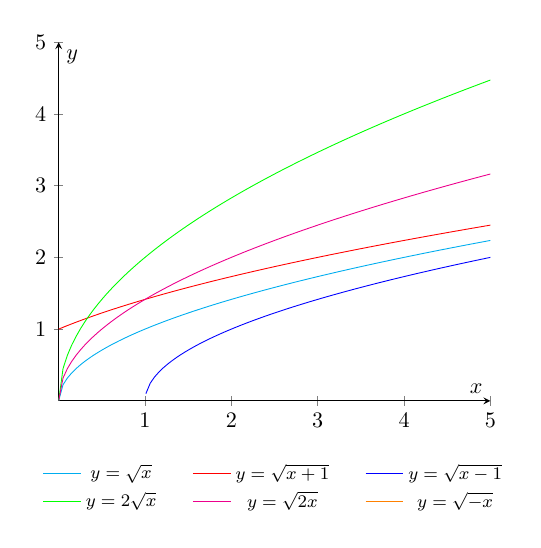
\begin{tikzpicture}[scale=0.8]
    \begin{axis}[
        axis lines=middle,
        xlabel=$x$,
        ylabel=$y$,
        xmin=0,
        xmax=5,
        ymin=0,
        ymax=5,
        xtick={0,1,2,3,4,5},
        ytick={0,1,2,3,4,5},
        legend pos=outer north east,
            legend style={
                draw=none,
                at={(0.5,-0.15)},
                anchor=north,
                legend columns=3,
                font=\footnotesize,
                /tikz/every even column/.append style={column sep=0.5cm},
            },
    ]
    \addplot[cyan, domain=0:5, samples=100] {sqrt(x)};
    \addlegendentry{$y = \sqrt{x}$}
    
    % Transformed Functions
    \addplot[red, domain=0:5, samples=100] {sqrt(x+1)};
    \addlegendentry{$y = \sqrt{x + 1}$}
    
    \addplot[blue, domain=0:5, samples=100] {sqrt(x-1)};
    \addlegendentry{$y = \sqrt{x - 1}$}
    
    \addplot[green, domain=0:5, samples=100] {2*sqrt(x)};
    \addlegendentry{$y = 2\sqrt{x}$}
    
    \addplot[magenta, domain=0:5, samples=100] {sqrt(2*x)};
    \addlegendentry{$y = \sqrt{2x}$}

    \addplot[orange, domain=0:5, samples=100] {sqrt(-x)};
    \addlegendentry{$y = \sqrt{-x}$}
    
    \end{axis}
    \end{tikzpicture}
    \end{center}
    \textbf{Definition ungerader Wurzelexponent}\\
    \textbf{Definitonsmenge}: $\mathbb{D} = \mathbb{R^+}$\\
    \textbf{Wertemenge}: $\mathbb{W} = \mathbb{R^+}$\\
    \textbf{Definition gerader Wurzelexponent}\\
    \textbf{Definitonsmenge}: $\mathbb{D} = \mathbb{R}$\\
    \textbf{Wertemenge}: $\mathbb{W} = \mathbb{R}$\\

    % Absolute Value Function: y = |x|

    \subsection*{Betragsfunktion}
    \begin{center}
    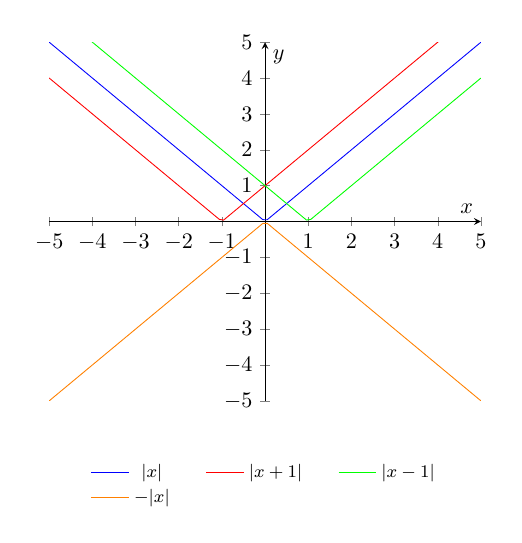
\begin{tikzpicture}[scale=0.8]
    \begin{axis}[
        axis lines=middle,
        xlabel=$x$,
        ylabel=$y$,
        xmin=-5,
        xmax=5,
        ymin=-5,
        ymax=5,
        xtick={-5,-4,-3,-2,-1,0,1,2,3,4,5},
        ytick={-5,-4,-3,-2,-1,0,1,2,3,4,5},
        legend pos=outer north east,
        legend style={
            draw=none,
            at={(0.5,-0.15)},
            anchor=north,
            legend columns=3,
            font=\footnotesize,
            /tikz/every even column/.append style={column sep=0.5cm},
        },
    ]
    
    \addplot[samples=100,blue]{abs(x)};
            \addlegendentry {$|x|$};
            \addplot[samples=100,red]{abs(x+1)};
            \addlegendentry {$|x+1|$};
            \addplot[samples=100,green]{abs(x-1)};
            \addlegendentry {$|x-1|$};
            \addplot[samples=100,orange]{-abs(x)};
            \addlegendentry {$-|x|$};
    
    \end{axis}
    \end{tikzpicture}
    \end{center}
    \begin{center}
        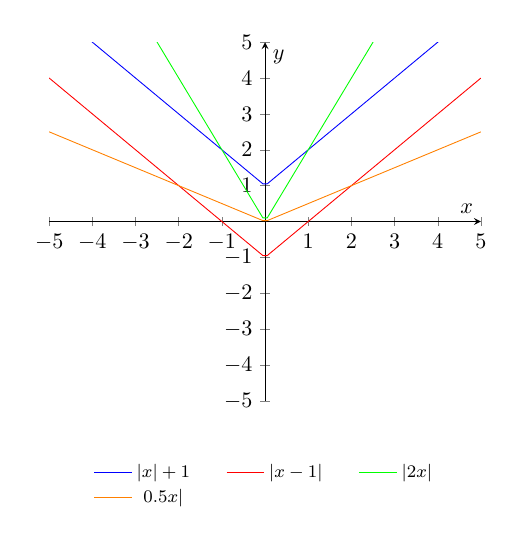
\begin{tikzpicture}[scale=0.8]
        \begin{axis}[
            axis lines=middle,
            xlabel=$x$,
            ylabel=$y$,
            xmin=-5,
            xmax=5,
            ymin=-5,
            ymax=5,
            xtick={-5,-4,-3,-2,-1,0,1,2,3,4,5},
            ytick={-5,-4,-3,-2,-1,0,1,2,3,4,5},
            legend pos=outer north east,
            legend style={
                draw=none,
                at={(0.5,-0.15)},
                anchor=north,
                legend columns=3,
                font=\footnotesize,
                /tikz/every even column/.append style={column sep=0.5cm},
            },
        ]
        
        \addplot[samples=100,blue]{abs(x)+1};
        \addlegendentry {$|x|+1$};
        \addplot[samples=100,red]{abs(x)-1};
        \addlegendentry {$|x-1|$};
        \addplot[samples=100,green]{abs(2*x)};
        \addlegendentry {$|2x|$};
        \addplot[samples=100,orange]{abs(0.5*x)};
        \addlegendentry {$0.5x|$};
        
        \end{axis}
        \end{tikzpicture}
        \end{center}

        \subsection*{Gebrochenrationale Funktionen}
      
        \textbf{Definitionsmenge}\\
         $\mathbb{D}_f = \mathbb{R}\setminus\{\text{Nullstellen der Nennerfunktion}\}$
        \subsubsection*{Senkrechte Asymptote}
        Eine senkrechte Gerade, der sich eine Kurve bei deren immer grösser werdender Entfernung vom Koordinatenursprung unbegrenzt nähert, heisst senkrechte Asymptote.\\
        \textbf{Bedingung}\\
        Bedingung für die Existenz einer senkrechten Asymptote ist, dass die Nennerfunktion (mindestens) eine Nullstelle hat:
        \textbf{Anleitung}
        Funktionsgleichung der Nennerfunktion gleich Null setzen: \\
        $f(x) = \frac{1}{x-1} \Longrightarrow x - 1 = 0$  \\
        Gleichung lösen: $x = 1$ \\
        Die senkrechte Asymptote verlauft durch x = 1.
         
        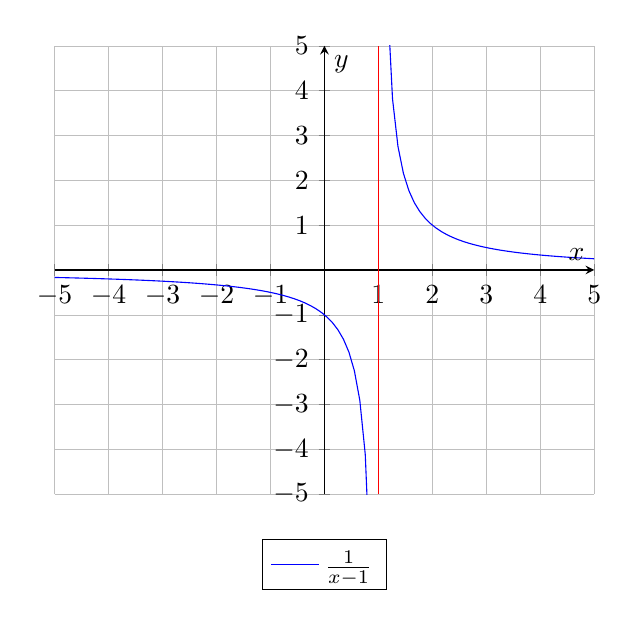
\begin{tikzpicture}%[scale=1.0]
            \begin{axis}[
                    xlabel=$x$,
                    ylabel=$y$,
                    xmax=5,
                    xmin=-5,
                    ymax=5,
                    ymin=-5,
                    axis x line=middle,
                    axis y line=middle,
                    legend style={at={(0.5,-0.1)},
                            anchor=north,legend columns=-1},
                    grid=major,
                    grid style={line width=.1pt, draw=gray!10},
                    major grid style={line width=.2pt,draw=gray!50},
                    xtick={-5,-4,-3,-2,-1,0,1,2,3,4,5},
                    ytick={-5,-4,-3,-2,-1,0,1,2,3,4,5},
                    samples=50
                ]
                \addplot[samples=100,domain=-5:5,blue,restrict y to domain=-15:15]{1/(x-1)};
                \addlegendentry {$\frac{1}{x-1}$};
                \draw[red] ({axis cs:1,0}|-{rel axis cs:0,0}) -- ({axis cs:1,0}|-{rel axis cs:0,1});
                \addlegendentry {$x=1$};
    
            \end{axis}
        \end{tikzpicture}\\
        \subsubsection*{Waagrechte Asymptote}
        Eine waagrechte Gerade, der sich eine Kurve bei deren immer groesser werdender Entfernung vom Koordinatenursprung unbegrenzt nähert, heisst waagrechte Asymptote.
        \textbf{Bedingung}\\
        Eine gebrochenrationale Funktion:
        \[y = \frac{{\color{red}a_n} x^{\fcolorbox{red}{white}{$n$}} + a_{n-1} x^{n-1} + \dots + a_1 x + a_ 0}{{\color{red}b_m} x^{\fcolorbox{red}{white}{$m$}} + b_{m-1} x^{m-1} + \dots + b_1 x + b_ 0}\]
        besitzt eine waagrechte Asymptote, wenn: \\
        Zählergrad < Nennergrad (n < m) dann: Die x-Achse ist die waagrechte Asymptote \\
        Zählergrad = Nennergrad (n = m) dann:  Die zur x-Achse parallele Gerade mit der Gleichung $y = {\color{red}\frac{a_n}{b_m}}$ ist die waagrechte Asymptote.
        \textbf{Anleitung}\\
        Zählergrad und Nennergrad bestimmen: \\
        Da der Zählergrad (0) kleiner ist als der Nennergrad (1), besitzt die gebrochenrationale Funktion eine waagrechte Asymptote.
        Waagrechte Asymptote berechnen: \\
        Wegen Zählergrad < Nennergrad ist die x-Achse die waagrechte Asymptote.
        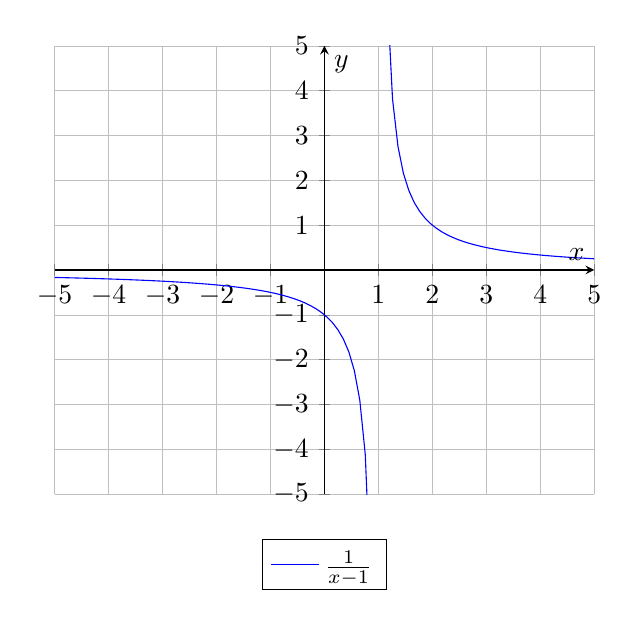
\begin{tikzpicture}%[scale=1.0]
            \begin{axis}[
                    xlabel=$x$,
                    ylabel=$y$,
                    xmax=5,
                    xmin=-5,
                    ymax=5,
                    ymin=-5,
                    axis x line=middle,
                    axis y line=middle,
                    legend style={at={(0.5,-0.1)},
                            anchor=north,legend columns=-1},
                    grid=major,
                    grid style={line width=.1pt, draw=gray!10},
                    major grid style={line width=.2pt,draw=gray!50},
                    xtick={-5,-4,-3,-2,-1,0,1,2,3,4,5},
                    ytick={-5,-4,-3,-2,-1,0,1,2,3,4,5},
                    samples=50
                ]
                \addplot[samples=100,domain=-5:5,blue,restrict y to domain=-15:15]{1/(x-1)};
                \addlegendentry {$\frac{1}{x-1}$};
            \end{axis}
        \end{tikzpicture}\\
    \normalsize
    

    \newpage
\end{multicols}

% Section Trigonometrie
\section*{Trigonometrie}
\begin{multicols}{3}

\small
\begin{multicols}{2}
\subsection*{Identitäten}

\textbf{Kofunktionen}
\begin{align*}
    & \sin(\frac{\pi}{2} - x) & = \cos x \\
    & \cos(\frac{\pi}{2} - x) & = \sin x \\
    & \tan(\frac{\pi}{2} - x) & = \cot x \\
    & \cot(\frac{\pi}{2} - x) & = \tan x \\
    & \sec(\frac{\pi}{2} - x) & = \csc x \\
    & \csc(\frac{\pi}{2} - x) & = \sec x
\end{align*}
\textbf{Symmetrie}
\begin{align*}
  \sin(-x) & = - \sin x \\
  \cos(-x) & = \cos x   \\
  \tan(-x) & = -\tan x
\end{align*}
\textbf{Doppelter Winkel}
\begin{align*}
  \sin(2x) & = 2 \sin x \cos x               \\
  \cos(2x) & = \cos^2 x - \sin^2 x           \\
           & = 2 \cos^2 x - 1                \\
           & = 1 - 2 \sin^2 x                \\
  \tan(2x) & = \frac{2 \tan x}{1 - \tan^2 x}
\end{align*}
\textbf{Halber Winkel}
\begin{align*}
  \sin \frac{x}{2} & = \pm \sqrt{ \frac{1 - \cos x }{2} } \\
  \cos \frac{x}{2} & = \pm \sqrt{ \frac{1 + \cos x }{2} } \\
  \tan \frac{x}{2} & = \frac{1 - \cos x }{\sin x}         \\
                   & = \frac{ \sin x }{ 1 + \cos x }
\end{align*}
\textbf{Exponent Reduktion}
\begin{align*}
  \sin^2 x & = \frac{1 - \cos 2x}{2}               \\
  \sin^4x  & = (\frac{1 - \cos 2x}{2})^2           \\
  \cos^2 x & = \frac{1 + \cos 2x}{2}               \\
  \cos^4x  & = (\frac{1 + \cos 2x}{2})^2           \\
  \tan^2 x & = \frac{1 - \cos 2x}{1 + \cos 2x}     \\
  \tan^4 x & =( \frac{1 - \cos 2x}{1 + \cos 2x})^2
\end{align*}
\textbf{Pythagoras}
\begin{align*}
  \sin^2 x + \cos^2 x & = 1        \\
  1 + \tan^2 x        & = \sec^2 x \\
  1 + \cot^2 x        & = \csc^2 x
\end{align*}
\textbf{Umkehrwert}
\begin{align*}
  \cot x & = \frac{1}{\tan x} \\
  \csc x & = \frac{1}{\sin x} \\
  \sec x & = \frac{1}{\cos x}
\end{align*}
\textbf{Quotient}
\begin{align*}
    \tan(x) = \frac{\sin(x)}{\cos(x)}\\
    \cot(x) = \frac{\cos(x)}{\sin(x)}
\end{align*}
\end{multicols}
\textbf{Summe und Differenz von Winkel}
\begin{align*}
  \sin(x + y) & = \sin x \cos y + \cos x \sin y             \\
  \sin(x - y) & = \sin x \cos y - \cos x \sin y             \\
  \cos(x + y) & = \cos x \cos y - \sin x \sin y             \\
  \cos(x - y) & = \cos x \cos y + \sin x \sin y             \\
  \tan(x + y) & = \frac{\tan x + \tan y}{1 - \tan x \tan y} \\
  \tan(x - y) & = \frac{\tan x - \tan y}{1 + \tan x \tan y}
\end{align*}
\textbf{Produkt zu Summe}
\begin{align*}
  \sin x \sin y & = \frac{1}{2}\big[\cos(x - y) - \cos(x + y)\big] \\
  \cos x \cos y & = \frac{1}{2}\big[\cos(x - y) + \cos(x + y)\big] \\
  \sin x \cos y & = \frac{1}{2}\big[\sin(x + y) + \sin(x - y)\big] \\
  \tan x \tan y & = \frac{ \tan x + \tan y }{ \cot x + \cot y }    \\
  \tan x \cot y & = \frac{ \tan x + \cot y }{ \cot x + \tan y }
\end{align*}
\textbf{Summe Zu Produkt}
\begin{align*}
  \sin x + \sin y & = 2 \sin \Big( \frac{x + y}{2} \Big) \cos \Big( \frac{x - y}{2} \Big)  \\
  \sin x - \sin y & = 2 \cos \Big( \frac{x + y}{2} \Big) \sin \Big( \frac{x - y}{2} \Big)  \\
  \cos x + \cos y & = 2 \cos \Big( \frac{x + y}{2} \Big) \cos \Big( \frac{x - y}{2} \Big)  \\
  \cos x - \cos y & = -2 \sin \Big( \frac{x + y}{2} \Big) \sin \Big( \frac{x - y}{2} \Big) \\
  \tan x + \tan y & = \frac{ \sin(x + y) }{ \cos x \cos y}                                 \\
  \tan x - \tan y & = \frac{ \sin(x - y) }{ \cos x \cos y}                                 \\
\end{align*}
\textbf{Additionstheoreme}
\begin{align*}
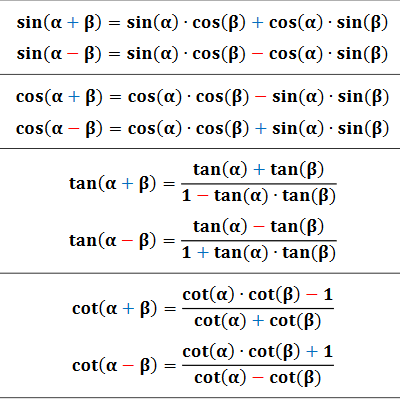
\includegraphics[scale=0.6]{trig/trig1.PNG}\\
\end{align*}
\textbf{Winkelfunktion des dreifachen winkel}
\begin{align*}
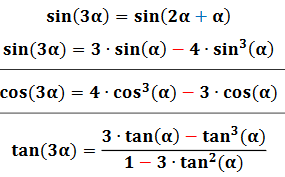
\includegraphics[scale=0.6]{trig/trig2.PNG}\\
\end{align*}
\newpage
\end{multicols}

% Section Vektoren
\section*{Vektoren}
\begin{multicols}{3}
\subsection*{Definition}
Ein Vektor ist durch Länge, Richtung und Orientierung eindeutig bestimmt.
\subsubsection*{Ortsvektor}
Ein Vektor, dessen Anfangspunkt im Ursprung O und dessen Endpunkt im Punkt A liegt, heißt Ortsvektor $\boldsymbol{\overrightarrow{OA}}$
von A.
\begin{equation*}
    A(x|y) \quad \Rightarrow \quad \overrightarrow{OA} = \begin{pmatrix} x \\ y \end{pmatrix}
\end{equation*}

\subsubsection*{Vektoraddition}
Vektoren lassen sich nur dann addieren, wenn sie gleicher Dimension und gleicher Art sind.
\begin{equation*}
    \vec{a}+\vec{b} = \begin{pmatrix} x_a \\ y_a\end{pmatrix}+\begin{pmatrix} x_b \\ y_b\end{pmatrix} = \begin{pmatrix} x_a+x_b \\ y_a+y_b\end{pmatrix}
\end{equation*}
\subsubsection*{Kommutativgesetz}
\begin{equation*}
    \vec{a}+\vec{b} = \vec{b}+\vec{a}
\end{equation*}
\subsubsection*{Assoziativgesetz}
\begin{equation*}
    (\vec{a}+\vec{b}) + \vec{c} = \vec{a} + (\vec{b}+\vec{c})
\end{equation*}

\subsubsection*{Vektorsubtraktion}
Vektoren werden subtrahiert, indem man ihre Komponenten subtrahiert:
\begin{equation*}
    \vec{a}-\vec{b} = \begin{pmatrix} x_a \\ y_a\end{pmatrix}-\begin{pmatrix} x_b \\ y_b\end{pmatrix} = \begin{pmatrix} x_a-x_b \\ y_a-y_b\end{pmatrix}
\end{equation*}

\subsection*{Skalar­multiplikation}
Wird ein Vektor $\vec{v}$ mit einem Skalar (einer reellen Zahl) $\lambda$ multipliziert, wird jede Komponente des Vektors mit dieser Zahl multipliziert:
\begin{equation*}
    \lambda \cdot \vec{v} = \lambda \cdot \begin{pmatrix} x \\ y \end{pmatrix} = \begin{pmatrix} \lambda \cdot x \\ \lambda \cdot y \end{pmatrix}
\end{equation*}
\subsubsection*{Misc}
Multipliziert man einen Vektor mit einem Skalar c, wird der Vektor – in Abhängigkeit des Wertes des Skalars – verlängert, verkürzt und/oder er ändert seine Orientierung.\\
$c > 1$: Der Vektor wird verlängert.\\
$0 < c < 1$: Der Vektor wird verkürzt.\\
$c < 0$: Der Vektor ändert seine Orientierung.\\

\subsection*{Betrag eines Vektors}
Die Länge eines Vektors heisst Betrag des Vektors.
\begin{equation*}
    \vec{v}= \begin{pmatrix} x \\ y \end{pmatrix} \Rightarrow \left|\vec{v}\right| = \sqrt{x^2 + y^2}
\end{equation*}

\subsection*{Einheitsvektor}
Ein Vektor der Länge 1 heisst Einheitsvektor.
\begin{equation*}
    \vec{a}^0 = \frac{1}{|a|} \vec{a}
\end{equation*}
\subsubsection*{Abstand zweier Punkte}
Verbindungsvektor berechnen und dann Länge des Vektors berechnen.
\subsection*{Skalarprodukt}
Das Skalarprodukt ist eine mathematische Verknüpfung, die zwei Vektoren eine Zahl (Skalar) zuordnet.
\begin{equation*}
    \vec{a} \circ \vec{b} = \begin{pmatrix} a_1 \\ a_2 \\ a_3 \end{pmatrix} \circ \begin{pmatrix} b_1 \\ b_2 \\ b_3 \end{pmatrix} = a_1 \cdot b_1 + a_2 \cdot b_2 + a_3 \cdot b_3
\end{equation*}
\subsubsection*{Kommutativgesetz}
\begin{equation*}
    \vec{a} \circ \vec{b} = \vec{b} \circ \vec{a}
\end{equation*}
\subsubsection*{Distributivgesetz}
\begin{equation*}
    \vec{a} \circ \left(\vec{b} + \vec{c}\right) = \vec{a} \circ \vec{b} + \vec{a} \circ \vec{c}
\end{equation*}
\subsubsection*{Gemischtes
Assoziativgesetz}
\begin{equation*}
    \left(k \cdot \vec{a}\right) \circ \vec{b} = k \cdot \left(\vec{a} \circ \vec{b}\right)
\end{equation*}
\subsection*{Winkel zwischen zwei Vektoren}

\begin{equation*}
    \cos\varphi = \frac{\vec{u}\circ\vec{v}}{\left|\vec{u}\right|\cdot\left|\vec{v}\right|} \qquad \Rightarrow \qquad \varphi = \cos^{-1}\left(\frac{\vec{u}\circ\vec{v}}{\left|\vec{u}\right|\cdot\left|\vec{v}\right|}\right)
\end{equation*}
Skalarprodukt berechnen, Beträge der Vektoren berechnen, Zwischenergebnisse in die Formel einsetzen und Formel nach Winkel auflösen.

\newpage

\end{multicols}

% Add more sections and formulas as needed

\end{document}
